\documentclass[a4paper,twoside]{article}

\usepackage{epsfig}
\usepackage{subcaption}
\usepackage{calc}
\usepackage{amssymb}
\usepackage{amstext}
\usepackage{hyperref}
\usepackage{amsmath}
\usepackage{amsthm}
\usepackage{booktabs}
\usepackage{multicol}
\usepackage{pslatex}
\usepackage{apalike}
\usepackage{SCITEPRESS}   


\begin{document}

\title{Scene Detection in \textit{De Boer} Historical Photo Collection}

\author{\authorname{Anonymized}
\affiliation{}
\email{}
}

\keywords{Digital History, Computer Vision, Scene Detection, Digital Heritage}

\abstract{This paper demonstrates how transfer learning can be used to improve scene detection applied to a historical press photo collection. After applying transfer learning to a pre-trained Places-365 ResNet-50 model, we achieve a Top-1 accuracy of .68 and a Top-5 accuracy of .89 on our data set, which consists of 132 categories. In addition to describing our annotation and training strategy, we also reflect on the use of transfer learning and the evaluation of computer vision models for heritage institutes.}

\onecolumn \maketitle \normalsize \setcounter{footnote}{0} \vfill

\section{INTRODUCTION}
\label{sec:introduction}

\noindent Computer vision algorithms have become capable of locating and identifying objects represented in images with high accuracy.
While this specific technology is commonplace in self-driving cars, drone technology, and the analysis of social media posts, its use for heritage institutes has only recently been growing~\cite{bhargav_deep_2019,bell_computing_2018,mager_visual_2020,niebling_analyzing_2020}. 
The possible benefits for heritage institutions range from automatically enriching collections, to improving search capabilities, or enabling large-scale analysis of visual collections. 
The latter is of particular interest for historians with an interest in the visual representations of the past.

While computer vision technology advanced rapidly in the last decade, most computer vision research focuses on use cases that require contemporary data as training material. 
Exceptions include art-historical research that relies on computer vision~\cite{madhu2019recognizing,bell2019ikonographie,offert2018images}. 
Training on contemporary material results in models not tuned to detect objects in heritage collections.
In other words, the models have difficulty detecting past representations of objects, which often looked noticeably different.
Moreover, the list of categories of objects in existing models are not always existent or relevant to heritage collections.
% 
In addition to objects changing, the visual medium itself has often-times changed, granting contemporary visual medium a different materiality. 
Compare, for example, a grainy black and white image of a traffic situation in the 1950s to a high-resolution color image taken with a zoom lens of a highway in 2020. 
In this instance, the cars will look different, but the improved technological capabilities of the camera also shaped the materiality of the picture. 
Models that are trained on millions of contemporary images do not have the sensitivity to deal with the color schemes and object representations in older images. 

One approach to counter this blind spot in models trained on contemporary data is to \textit{fine-tune} their performance by feeding them with historical
material.
This method builds upon the categories existent in the modern data sets. 
However, these categories do not always map onto the categories present in the collections of heritage institutes, or they do not align with the search interests of users of such heritage collections.
%
Another approach is \textit{transfer learning}, which adds new categories to existing models, which are trained using the historical material that has been annotated with these new categories. 
Because the models have already been pre-trained with large collections of images, we often only require a small number of images to learn a new category.  
Of course, this depends on the visual complexity of the category and the diversity present in the training data for that category. 
In other words, an object that always looks the same is easier to learn than one that shared visual aspects but also differs considerably.

Existing research that applies computer vision methods to historical photographs looks into automatically dating images~\cite{Palermo_2012}, matching images taken from different viewpoints~\cite{maiwald2019generation}, photogrammetric analysis of images~\cite{maiwald2017photogrammetric}, and the classification of historical buildings~\cite{llamasClassificationArchitecturalHeritage2017}.

As part of this research, we set out to discover what type of computer vision tasks were seen as most relevant in the context of heritage institutions. For this purpose, we conducted fourteen interviews with digital humanities experts, visitors of historical archives, and heritage experts.\footnote{Due to the Covid-19 pandemic, we had to conduct these interviews virtually. 
We originally intended to invite more people in person to the archive to conduct face-to-face interviews.}
We discussed several computer vision tasks, from which the respondents showed the most interest in object and scene detection, with a specific interest in tracing buildings. 
Other tasks such as the estimation of group sizes, facial emotion detection, detection of logos, and posture estimation, the respondents deemed less relevant.

This paper focuses on one particular computer vision task: scene detection. 
This task tries to describe ``the place in which the objects seat'', rather than classifying the object depicted on an image, or locating particular objects in a picture by drawing bounding boxes around them~\cite{zhou_places_2018}. 
More specifically, this paper applies transfer learning to Places-365, a scene detection model trained on contemporary data. 
We reflect on creating training data, the training strategy, as well as the evaluation of the model. 
Finally, we discuss the benefits of this type of computer vision algorithm for heritage institutes and visual archives.
Rather than merely detecting objects, the ability to search for images based on the scene represented in them is a useful feature for heritage institutions, especially since this information is often not included in the metadata. 
Using such information, historians could examine the representations of particular scenes, for example, protests, at scale. 

\section{DATA}
\noindent This data set for this study is the photo collection of press agency \textit{De
  Boer} for the period 1945-2004.\footnote{This data has been kindly provided by the
  \textit{Noord-Hollands Archief}.}
The \textit{De Boer} collection focuses on national and regional events, although over time the collection's focus gradually shifted to the region Kennemerland.
This region, just north of Amsterdam, includes cities such as Haarlem, Zandvoort, Bloemendaal, and Alkmaar.
%
The value of the collection was recognized locally, nationally, and
internationally.  In 1962, the founder of the press photo agency, Cees de Boer,
was awarded the World Press Photo and the Silver Camera (\textit{Zilveren
  Camera}).
He won the World Press Photo for a picture showing Dutch singer Ria Kuyken being attacked by a young bear in a circus.
Seven years later, Cees' son Poppe won the national photojournalism award. 
The photo collection depicted a wide range of events, ranging from the first and only show
of \textit{The Beatles} in the Netherlands in Blokker---a small village just north of Amsterdam, the arrival of Martin Luther King in 1964 (see Figure~\ref{fig:example}), to the opening of restaurants, and sports events.
The photo press agency was one of the main providers of pictures to the regional newspaper \textit{Haarlems Dagblad}.

\begin{figure}
	\centering
 	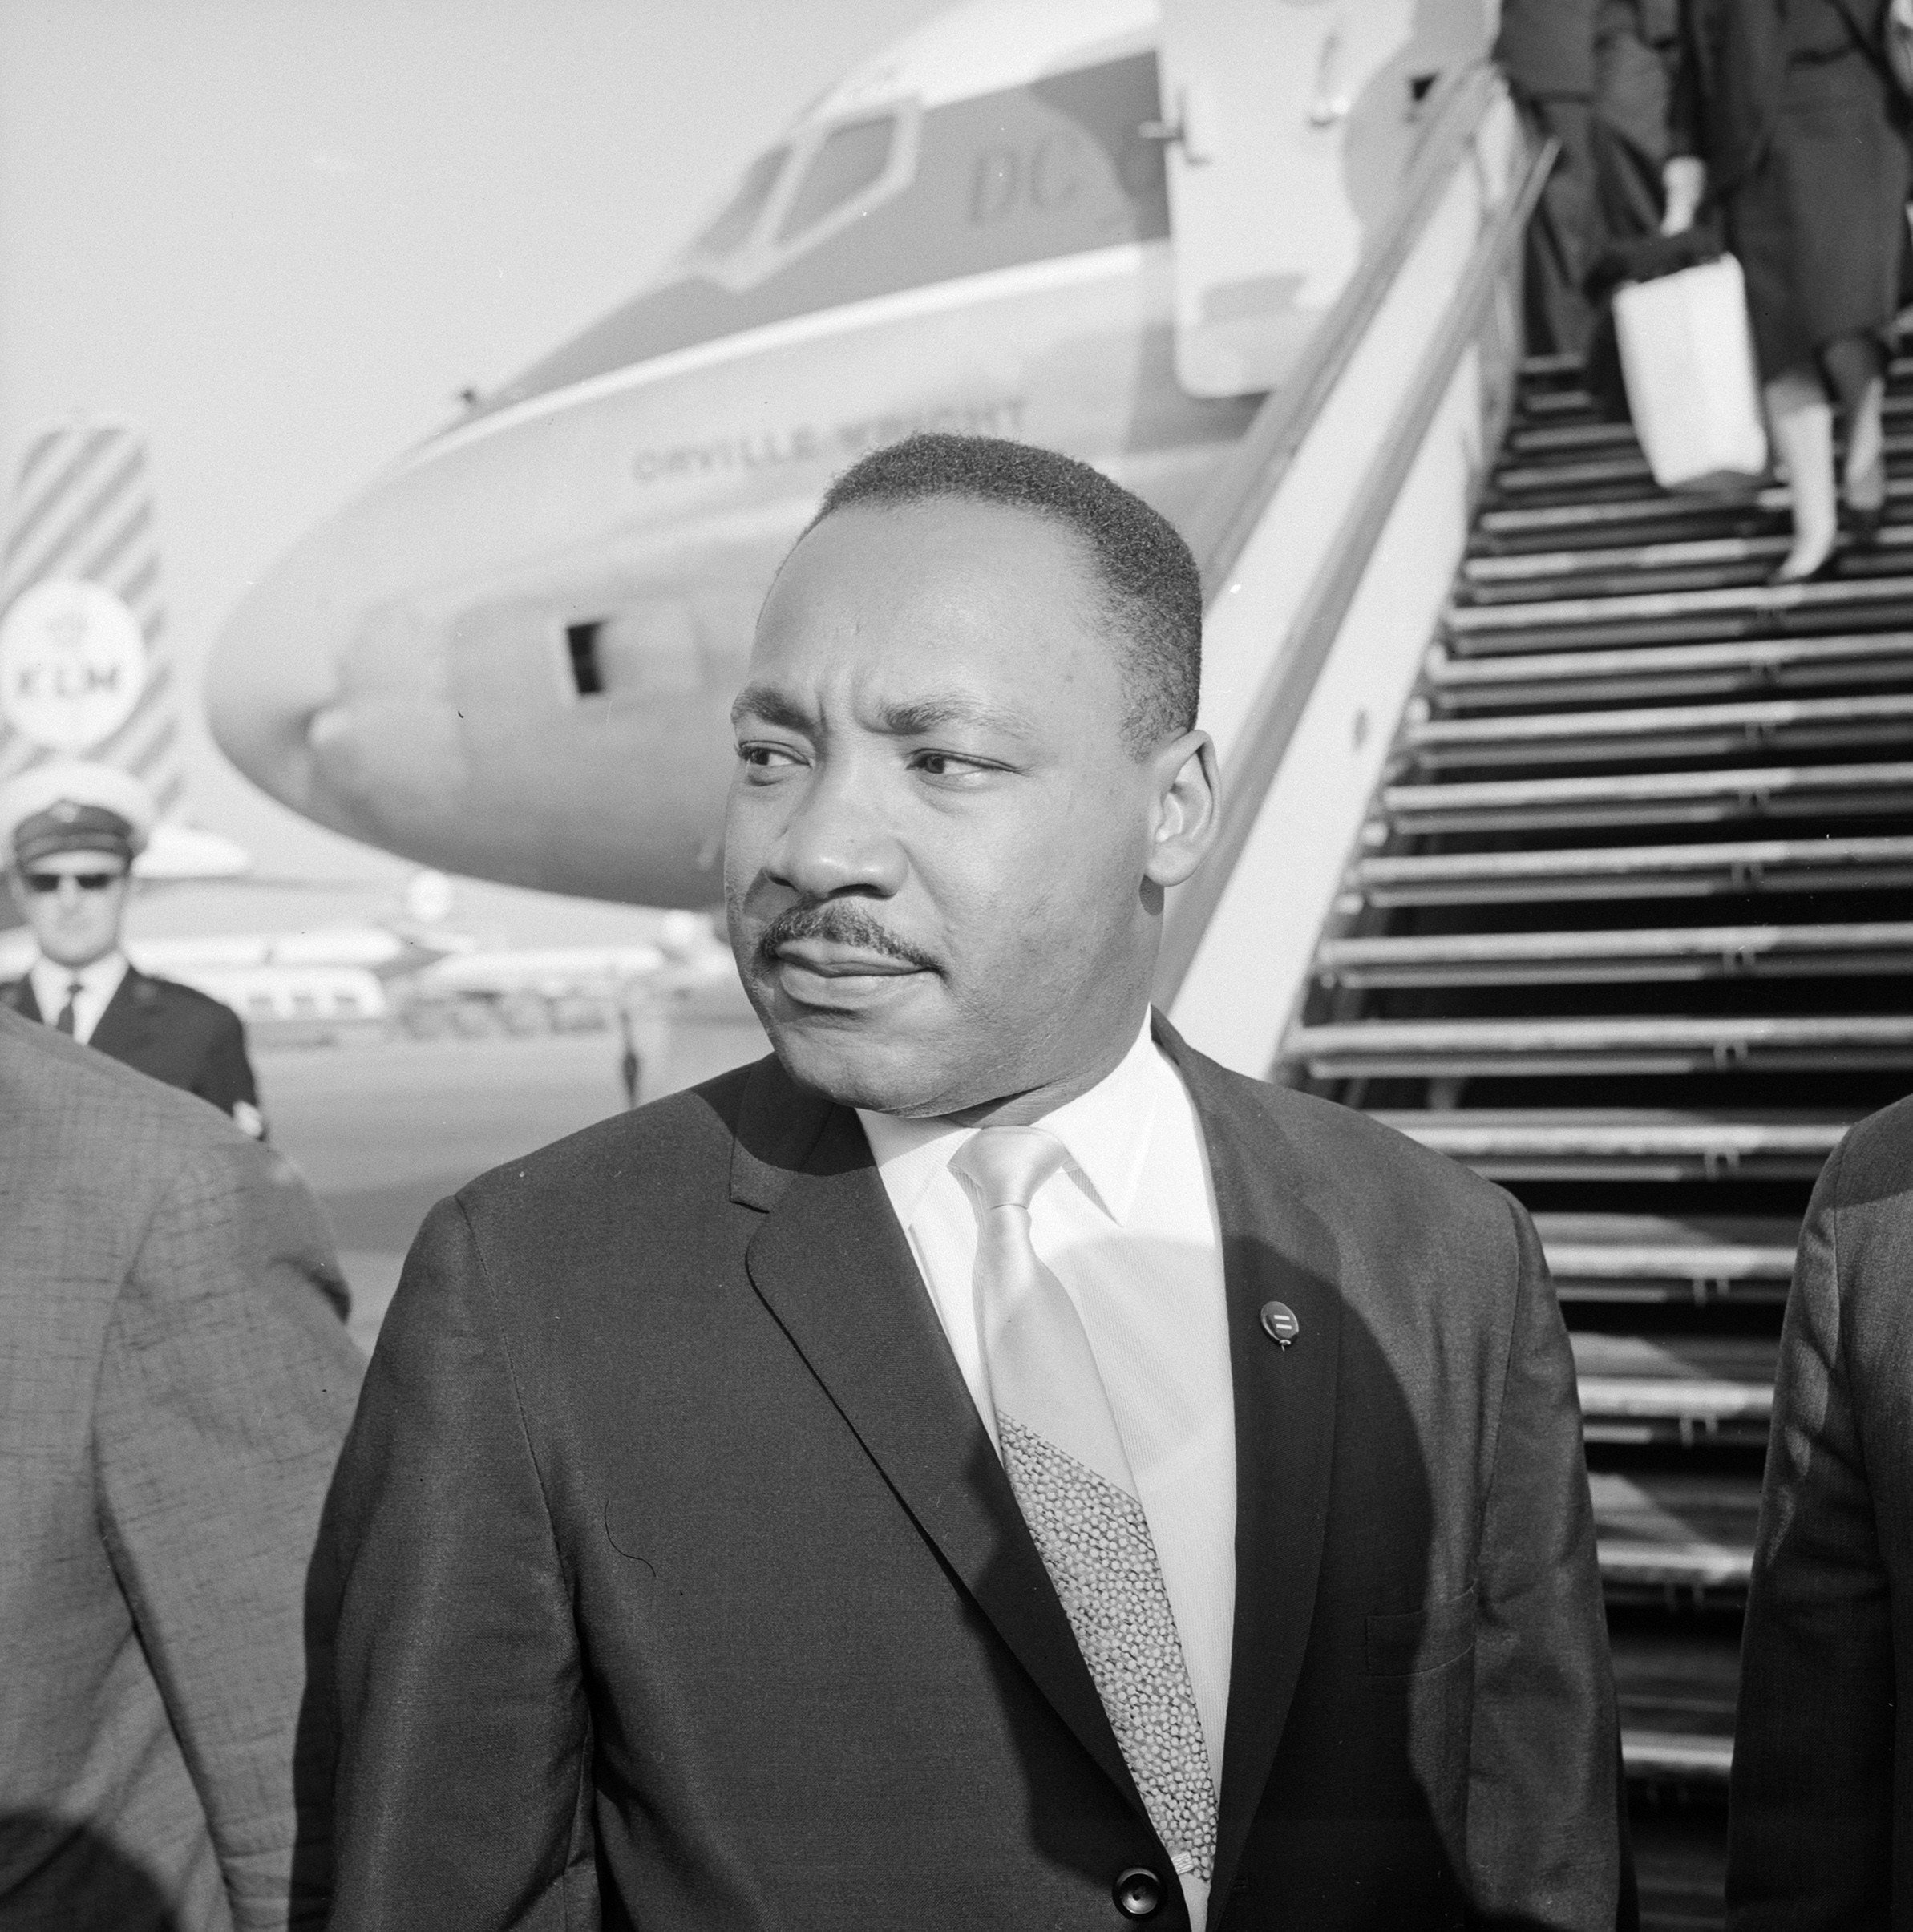
\includegraphics[width=\linewidth]{figures/MLK.jpg}
 	\caption{Arrival of Martin Luther King Jr. at Schiphol Airport, August 15, 1964. Taken from \emph{De Boer} Collection}
 	\label{fig:example}
\end{figure}

The photo collection consists of approximately two million negatives accompanied with metadata for the period 1945-2004.
The metadata is extracted from physical topic cards and logs kept by the photo agency.
On approximately nine thousand topic cards with over a thousand unique topics, the agency detailed what was depicted in the pictures. 
For the period 1952-1990, these logs have been transcribed using volunteers.\footnote{\url{https://velehanden.nl/projecten/bekijk/details/project/ranh}}

The archive is currently in the process of digitizing the two million negatives and linking these to the already-transcribed metadata.\footnote{\url{https://velehanden.nl/projecten/bekijk/details/project/ranh_tagselection_deboer}}
At the moment of this pilot study, the archive has only digitized a selection of images. 
This pilot study explores whether transfer learning can be applied to the data and how we should categorize and label the data. 
During the larger digitization project, we will use the annotation strategy developed in this study to label a selection of images to further improve the scene detection model. 
This model will also be used to automatically label images or detect images that are more difficult to label and which require human annotators.
The enriched photo collection will be used to improve the search functionality of the archive. 
The labeled data and resulting model will be made publicly available to serve as a starting point for other historical photo collections that want to apply computer vision to their collection.

For this pilot study, we relied on a subset of 2,545 images that had already been digitized by the \emph{Noord-Hollands Archief}. 
Together with archivists and cultural historians, we constructed scene categories for these images.\footnote{In the Appendix, we added annotation guidelines, which will be used for the annotation of the further data set.} 
We used the categorization scheme used in Places-365 as a starting point. 
As the name implies, this scheme contains 365 categories of scenes, ranging from `alcove' to `raft'.\footnote{An overview of the categories can be found here: \url{http://places2.csail.mit.edu/explore.html}} 
We combined the categories in Places-365 with categories from the catalog cards that \textit{De
  Boer} used. 
These catalog cards could not be linked to the categorization scheme directly, because these cards often contain categories that are too specific or categories that were represented visually. 
These categories could only be inferred from contextual information but not from the image itself. 
During the process, we encountered that the creation of categories is always a trade-off between specificity and generalization. 
In making these categories, we kept in mind whether there remained a historical and visual consistency in the categories and whether the category would be of use for users of the collection. 
At the same time, we had to make sure we were not too specific, which would impact the amount of training data. 

During the annotation process, we noticed the difficulty in distinguishing between scenes that were characterized by a particular object and scenes defined by the location or the action performed in the image.
For example, the images in Figure~\ref{fig:examples_objects} contain specific objects, while the images in Figure~\ref{fig:examples_scenes} depict scenes.
Still, the images in the latter also contain objects such as flags, wreaths, cranes, and trees that are not necessarily exclusive to a specific scene.
This particular challenge is also discussed by developers of scene detection data sets.
The developers of the SUN database, for example, describe how scenes are linked to particular functions and behaviors, which are closely tied to the visual features that structure the space.
In the case of large rooms or spacious areas, these allow for different types of behavior, opening up the possibility for different scene categories~\cite{xiao2010sun}. 
Moreover, there are instances of large inter-class similarity between scenes, for instance, between the categories `library' and `bookstore'.
At the same time, we find large intra-class variations, in which the depicted scenes that belong to one category are actually quite diverse~\cite{xie_scene_2020}.

After annotation, we used an initial baseline model to correct incorrectly annotated images. 
During the annotation process of the larger dataset, we will iteratively evaluate the training categories and possibly add new categories and merge or remove existing ones.
%
\begin{figure}
 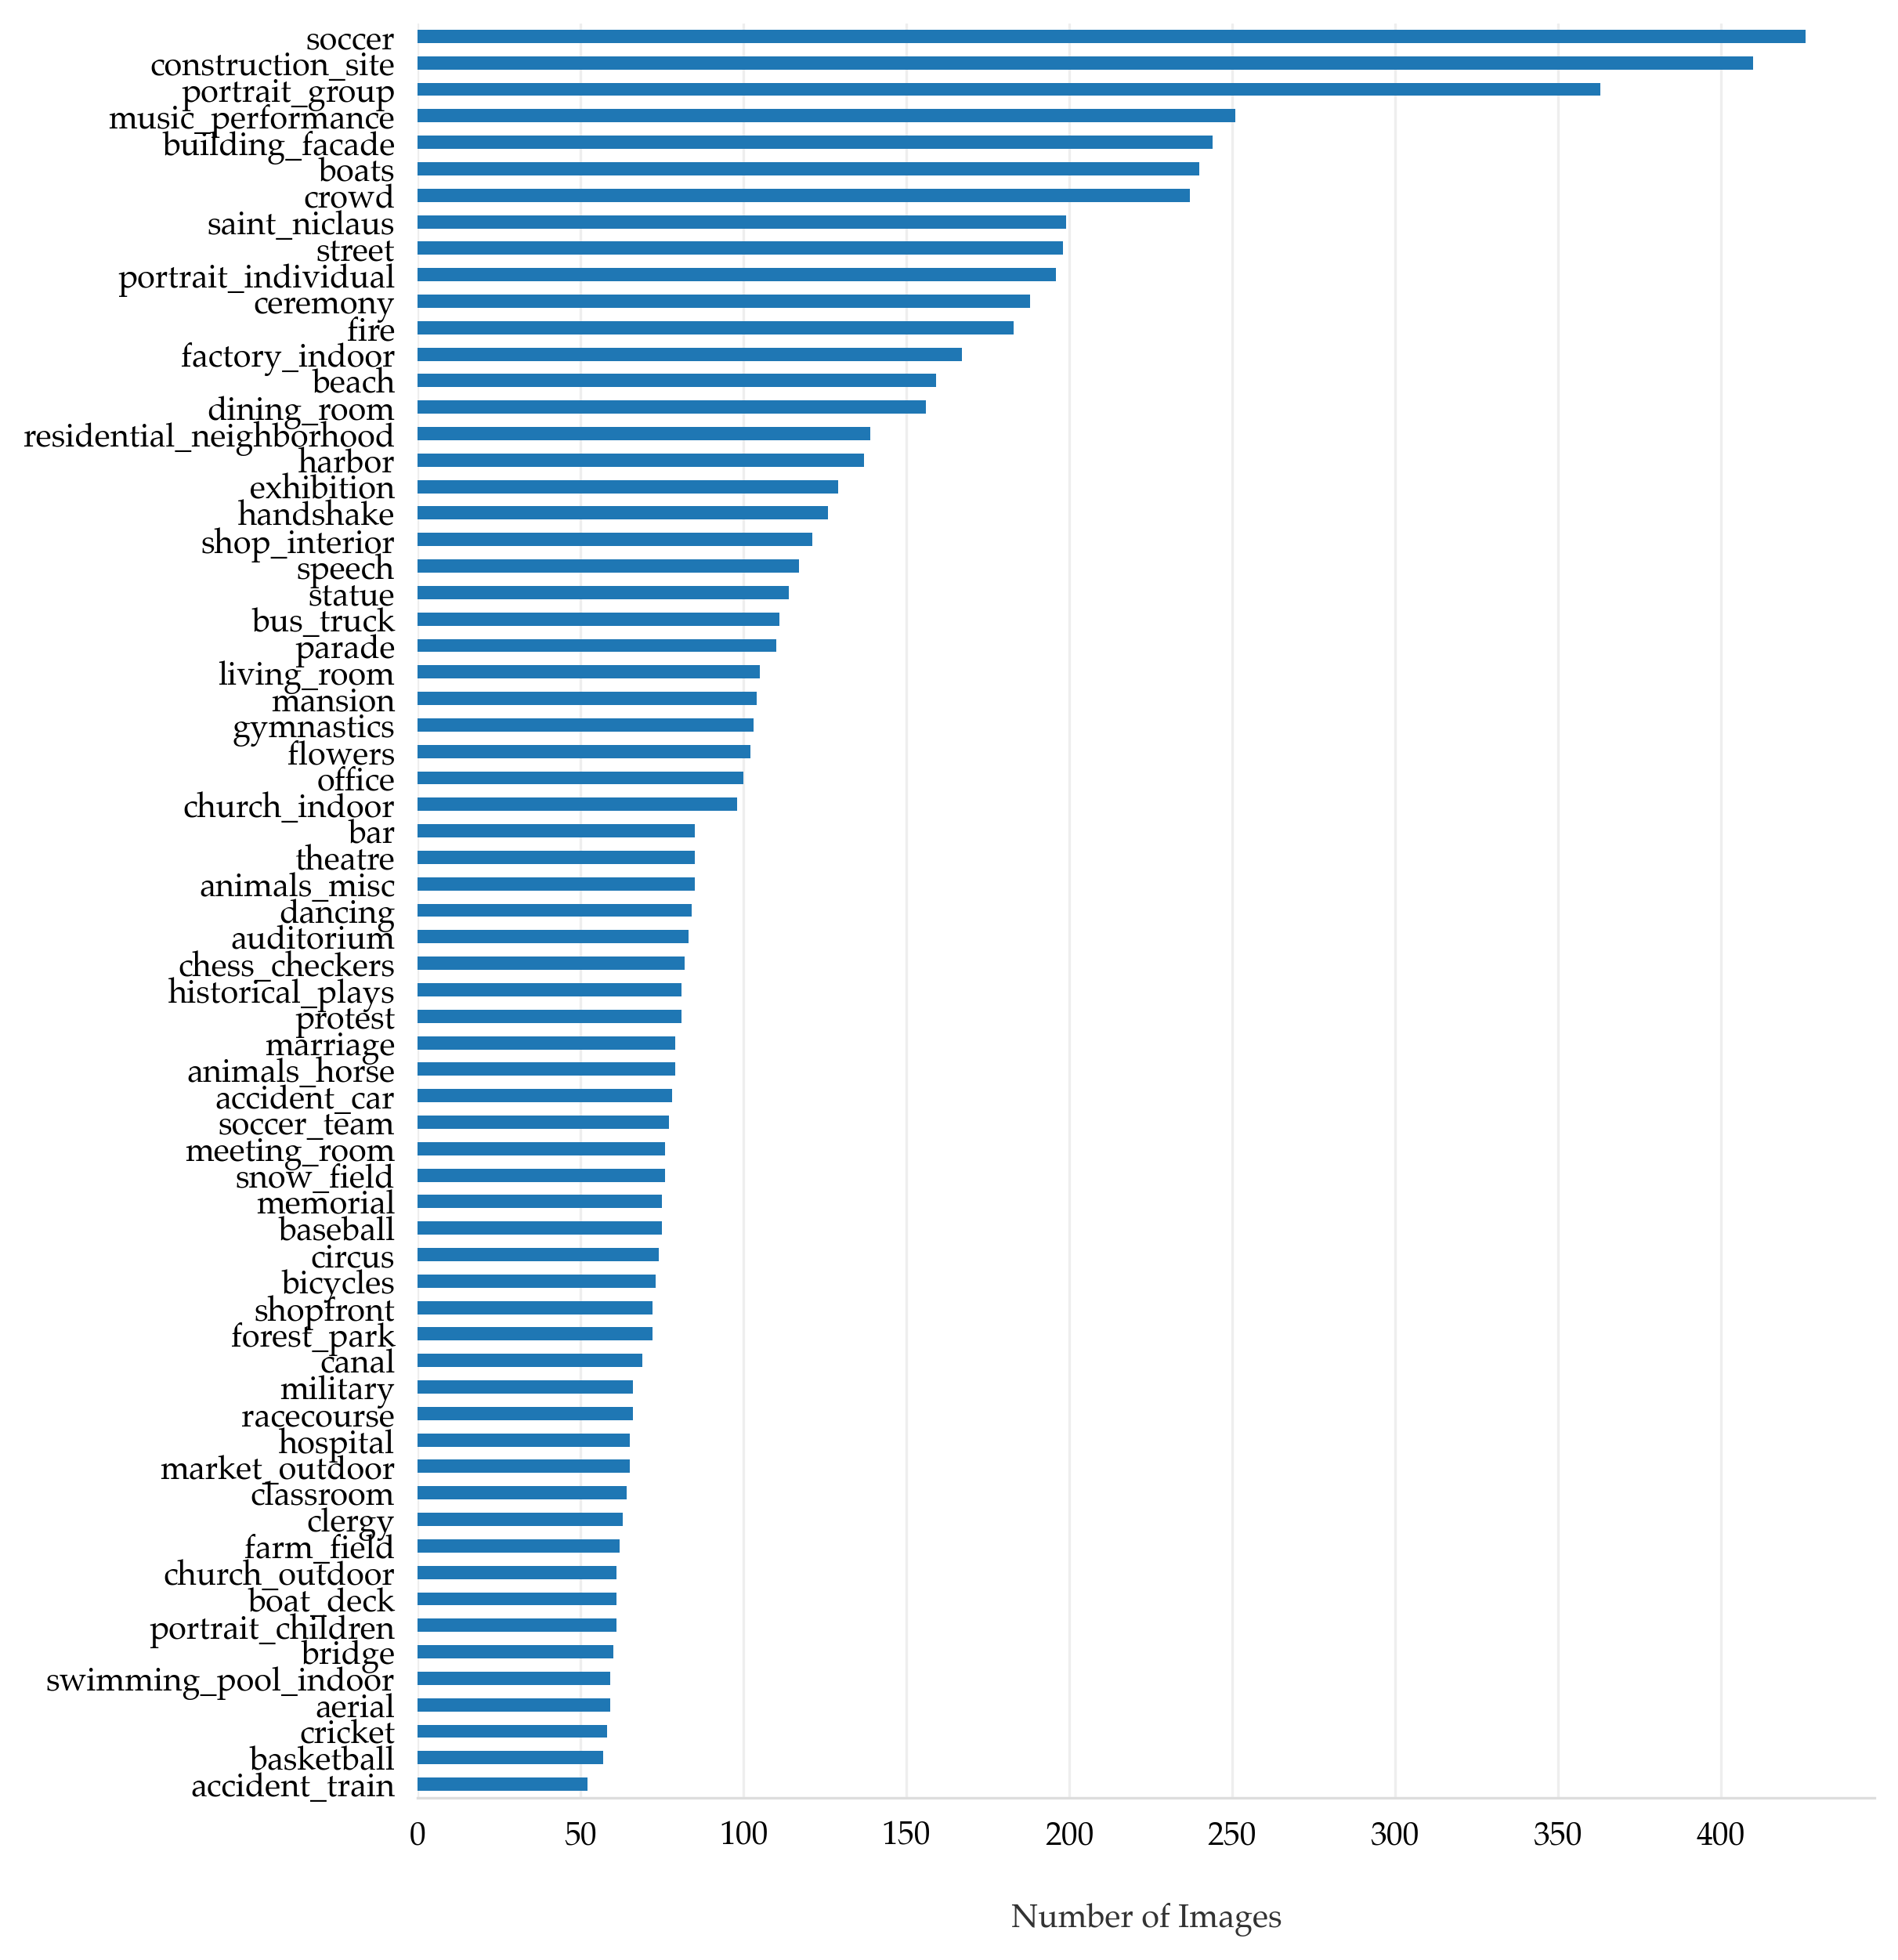
\includegraphics[width=\linewidth]{figures/categories.png}
 \caption{Distribution of categories ($N \geqslant50$) in the training set.}
 \label{fig:categories}
\end{figure}
%
Our resulting dataset includes 115 unique categories that can be found along with their descriptions in the Appendix.  
The distribution of the categories in our training set is heavily skewed and long-tailed (Figure~\ref{fig:categories}). 
For training, we removed categories with less than twenty images, this included categories such as: `houseboat', `castle', and `campsite'. 
However, we intend to again include these categories when we are annotating the newly digitized photographs.
The categories `soccer' and `construction site', for instance, are very well represented, while most others appeared much more infrequently. 
Even though transfer learning can produce accurate results with few training examples, more training data, especially in categories with greater visual variations, is to be preferred. 



\section{SCENE DETECTION}
\label{sec:scene_detection}
\noindent The authors of the Places-365 data set describe a scene as an ``environment(s) in the world, bounded by spaces where a human body would fit''~\cite{zhou_places_2018}. 
Scene detection is aimed at detecting such an environment, or scene, from visual material. 
Humans can quickly recognize the functional and categorical properties of a scene while ignoring the objects and locations in a scene~\cite{oliva_modeling_2001}. 
Still, this does not mean that humans recognize scenes in an unequivocal manner. 
Contextual factors that are necessarily part of the image aid humans in describing scenes depicted in the image.  
Users of heritage collections rely on search not only to discover for representations of particular objects~\cite{petras2017europeana,clough2017europeana}.
Especially in the context of press photography, photographs often captured a particular historical event or setting.
Press photos are highly diverse and more often than not contain more groups of people or objects placed in a particular setting.

In the \emph{De Boer} collection, we find depictions of scenes, such as memorials, construction sites, or parades (see Figure~\ref{fig:examples_scenes}). 
Even though these events are characterized by the presence of particular objects, in many cases, they cannot be described by just a single object or person.
%
At the same time, the collection also includes images that can accurately be described by a single object (see Figure~\ref{fig:examples_objects}). 
Scene detection, however, is also able to learn such representations. 

\begin{figure}
\center
 \begin{subfigure}[b]{0.33\textwidth}
    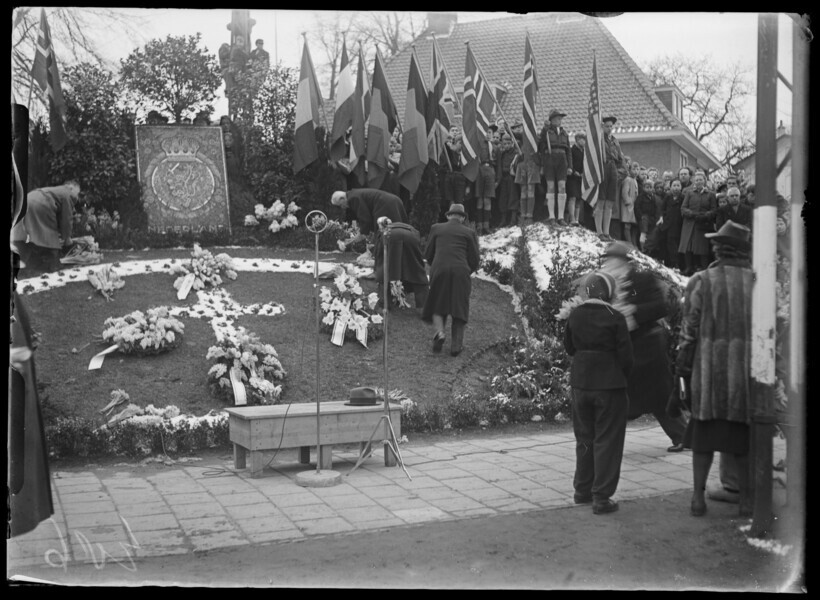
\includegraphics[width=\textwidth]{figures/memorial.jpg}
    \caption{Memorial}
    \label{fig:examplesa}
     \vspace{0.5em}
 \end{subfigure}
 %
 \begin{subfigure}[b]{0.33\textwidth}
    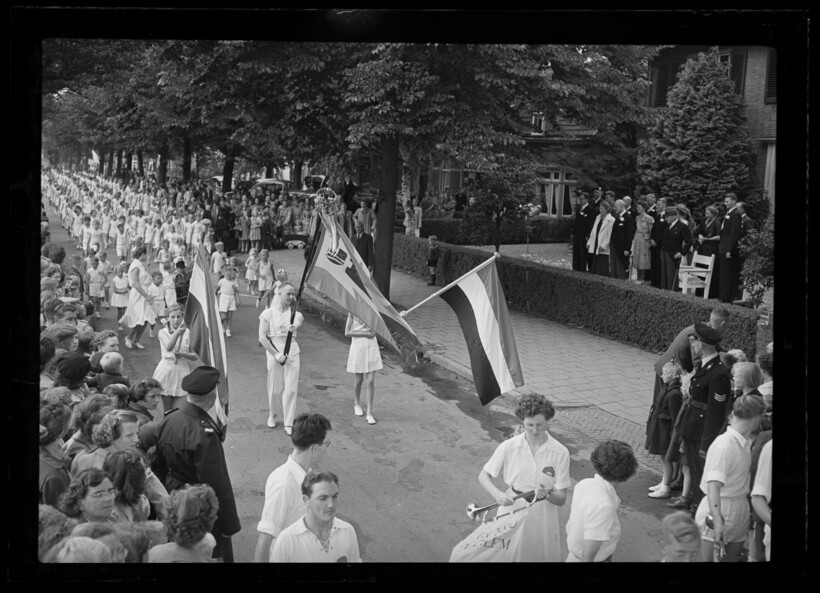
\includegraphics[width=\textwidth]{figures/parade.jpg}
    \caption{Parade}
    \label{fig:examplesb}
     \vspace{0.5em}
 \end{subfigure}
 %
 \begin{subfigure}[b]{0.33\textwidth}
    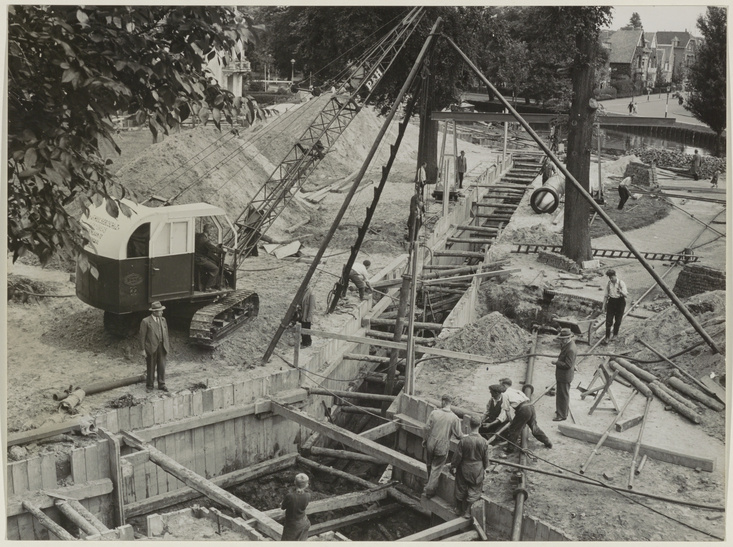
\includegraphics[width=\textwidth]{figures/construction_site.jpg}
    \caption{Construction Site}
    \label{fig:examplesc}
     \vspace{0.5em}
 \end{subfigure}
  \caption{Three photographs with scene labels from \textit{De Boer} collection.}
  \label{fig:examples_scenes}
\end{figure}

\begin{figure}
\center
 \begin{subfigure}[b]{0.33\textwidth}
    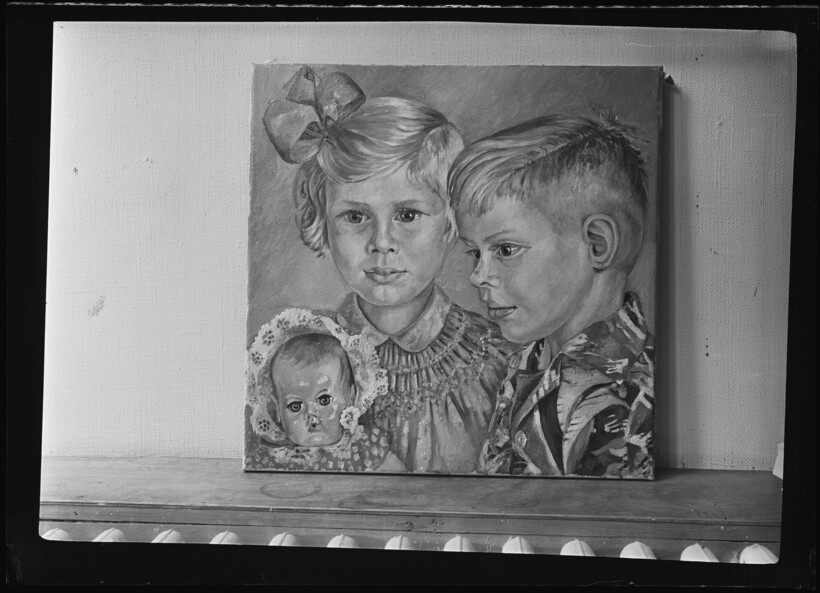
\includegraphics[width=\textwidth]{figures/artwork.jpg}
    \caption{Artwork}
    \label{fig:examplesa}
     \vspace{0.5em}
 \end{subfigure}

 %
 \begin{subfigure}[b]{0.33\textwidth}
    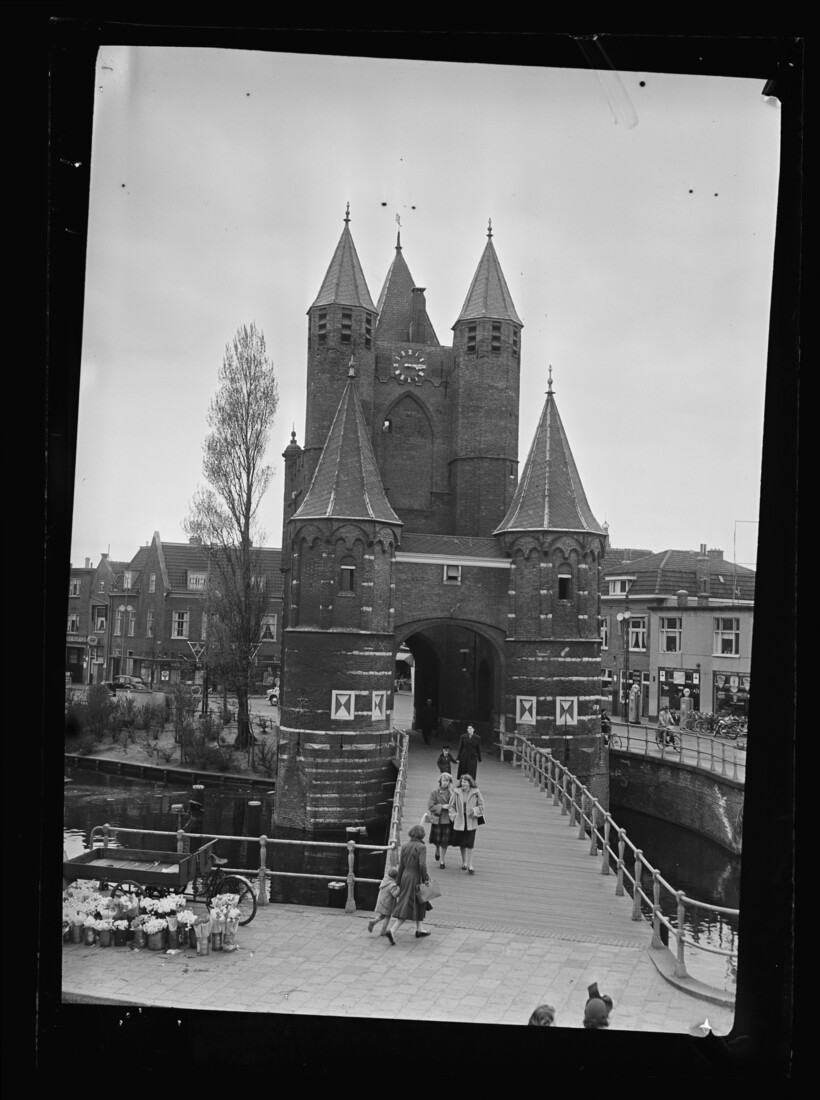
\includegraphics[width=\textwidth]{figures/castle.jpg}
    \caption{Castle}
    \label{fig:examplesb}
     \vspace{0.5em}
 \end{subfigure}
 %
 \begin{subfigure}[b]{0.33\textwidth}
    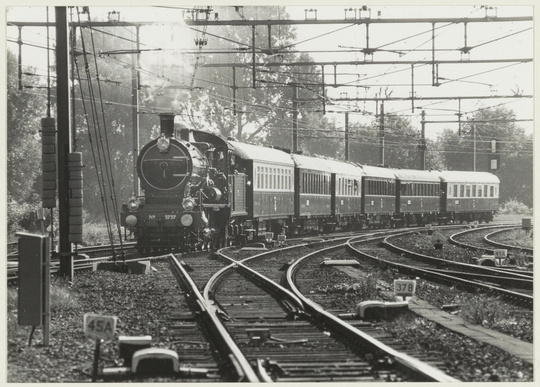
\includegraphics[width=\textwidth]{figures/train.jpg}
    \caption{Train}
    \label{fig:examplesc}
 \end{subfigure}
  \caption{Three photographs characterized by a central object from \textit{De Boer} collection.}
  \label{fig:examples_objects}
   \vspace{0.5em}
\end{figure}


We decided to not focus on object detection and the segmentation of possible objects, but rather to focus on the image as a whole using scene detection. 
The category schemes in existing object detection models were not directly applicable to the photographs in this collection. 
Using existing object detection models did not yield useful categories. 
For example, for a picture of a shopping street, object detection would identify people, bags, and perhaps a traffic light.
To be able to detect objects represented in our photo collection, we would need to draw bounding boxes around these objects and annotate them, which would prove to be a very time-consuming task. 
Nevertheless, in future work, we would like to explore the development of a framework that would provide historical descriptions based on the relationship between different objects in an image. 

\subsection{Transfer Learning}
\label{sec:transfer_learning}
For the adaptation of existing scene detection models to our data set, we turn to transfer learning~\cite{rawat_deep_2017}. 
This method refers to using ``what has been learned in one setting [...] to improve generalization in another setting''~\cite{goodfellow_deep_2016}. 
In our case, we use what has been learned about scenes captured in the Places-365 models to learn how to detect the scenes in our training data using our categorization scheme. 
Rather than training a model from scratch, transfer learning is known for reaching good accuracy in a relatively short amount of time. 
Basically, we build upon the information already stored in the places model, which is based on millions of labeled images.\footnote{for code and data see: \url{https://github.com/melvinwevers/hisvis}}

As a starting point, we use a ResNet-50 model---a convolutional neural network of fifty layers--- trained on the Places-365 dataset.\footnote{\url{https://github.com/CSAILVision/places365}} 
This dataset consists of ~1.8 million images from 365 scene categories.
The Places-365 data set builds upon the SUN database, consisting of 899 categories with short descriptions.\footnote{\url{https://groups.csail.mit.edu/vision/SUN/}} 
For our annotation guidelines, we used the SUN descriptions as a starting point. 
Given that our data set consists primarily out of black and white images, it is worth noting that this type of image was excluded from the SUN data.
Next, we create a random validation set, containing twenty percent of the training images. 
We use this validation set, to estimate the model's performance in terms of accuracy and its fit.
In the context of a heritage institute, scene detection is a meaningful task. 

Applied to the Places-365 validation data set, the Places-365 ResNet-50 model reaches a 54.74\% top-1 accuracy and 85.08\% top-5 accuracy.
Top-1 accuracy refers to the percentage of images where the predicted label with the highest probability matches the ground-truth label.
Top-5 accuracy calculates whether the ground-truth label is in the top-five predicted labels. 
Because of the ambiguity between scene categories, top-5 accuracy is generally seen as a more suitable criterion than top-1 accuracy~\cite{zhou_places_2018}. 
The Places-365 model outperforms the widely-used ImageNet-CNN on scene-related data sets, underscoring the benefit of using tailor-made models for scene detection over more generic models, such as ImageNet. Due to its performance on the places-365, we also turned to the ResNet-50 implementation. We have also experimented with simpler model architectures, but these were less able to capture the complexity of the images. 

For our study, we load a pre-trained Places-365 model, which we then tune to our categories using the deep learning framework Fast.AI~\cite{howard2018fastai}. 
We transfer learn using the One-Cycle method, an efficient approach to setting hyper-parameters (learning rate, momentum, and weight decay), which can lead to faster convergence~\cite{smithDisciplinedApproachNeural2018a}. 

To account for the unevenly distributed and often small number of training data and to prevent overfitting, we experiment with different data augmentation methods, including image transformation, label smoothing, MixUp, and CutMix. 
Overfitting refers to the model adapting too closely to the training data, making it less suitable for working with images the model was not trained on. 
The image transformations, in this case, include, flipping, rotating, and zooming of the source image. 
These transformations increase the number of training images the model sees and makes it harder for the model to overfit to a particular image. 
Labels Smoothing adds a small amount of noise to the one-hot encoding of the labels, making it more difficult for the model to be confident about the prediction. 
This reduces overfitting and improves the generalizability of the model~\cite{szegedyGoingDeeperConvolutions2014}.

MixUp and CutMix are two relatively recent data augmentation techniques. 
MixUp basically overlays two different images with different labels. 
For example, one can have an image of a cat with an overlay of a dog. 
This makes it more difficult for the model to determine what's in each image. 
The model has to predict two labels for each image as well the extent to which they are `mixed'~\cite{zhangMixupEmpiricalRisk2018}. 
%
CutMix is an extension of a random erasing technique that has often been used in data augmentation. 
In random erasing, a random block of pixels is removed from the image, making it harder for the model to learn the image. 
CutMix cuts and pastes random patches of pixels between training images. 
The labels are also mixed proportionally to the area of patches in the training image. 
CutMix pushes the model to focus on the less discriminative parts of an image, making it suitable for object detection~\cite{yunCutMixRegularizationStrategy2019}.
The downside of MixUp and CutMix can be that they make it too difficult for the model to detect features, causing underfitting. 

We train the model for a maximum of 35 epochs, with early stopping at five epochs monitoring changes in validation loss. 
To account for underfitting, we experimented with varying the $\alpha$ parameter of MixUp and CutMix, which controls how much of the augmentation is applied. 
Too much of the augmentation would make it too difficult for the model to extract generalizable features. 
Training a model is finding a balance between underfitting and overfitting, which is dependent on the size and complexity of the training data. 
In the domain of cultural heritage, we are often working with limited sets of annotated training material, making it worthwhile to examine to what extent transfer learning can be applied and how we can cope with overfitting to these limited sets of data. 
In our use case, we want to model to classify unseen data, which requires a model that can generalize.

\section{RESULTS}
\noindent Our baseline model which only uses image transformations achieves a top-1 accuracy of 0.62 and a top-5 accuracy of 0.88 (see Table~\ref{tab:results}). 
Adding MixUp with a low $\alpha$ (0.2) and Label Smoothing slightly improves the top-1 accuracy to 0.68, but these augmentations have no effect on the top-5 accuracy. 
The addition of CutMix and Label Smoothing has a similar effect with a Top-1 accuracy of 0.67. 
It is noteworthy that the baseline model already achieves good results, which underscores the power of transfer learning and the use of the Places-365 model as a starting point for more specific scene detection tasks. 
We can see that in almost nine out of ten cases, the correct result can be found in the top 5 results. 
For our larger data set, we will again explore to what extent MixUp and CutMix can boost the performance of the model.

\begin{table}[]
\small
\caption{Training Results}
\label{tab:results}
\begin{tabular}{lll}
\toprule
                & Top 1-Acc & Top 5-acc \\
\midrule
Baseline + Aug      &   \underline{\textbf{0.62}}    &  \underline{\textbf{0.88}}      \\
Label Smoothing (LS) &   0.61       &   0.87       \\
MixUp (0.2)     &  0.62        &     0.86 \\
MixUp (0.2) + Aug & 0.63 & 0.87 \\
MixUp (0.2) + Aug + LS  & \underline{\textbf{0.68}}   & \underline{\textbf{0.89}}\\
MixUp (0.3)     &  0.63        &     0.88 \\
MixUp (0.3) + Aug & 0.61 & 0.87 \\
MixUp (0.3) + Aug + LS  & 0.60   & 0.86 \\
MixUp (0.4)  &  0.67        &     0.89 \\
MixUp (0.4) + Aug & 0.61 & 0.86 \\
MixUp (0.4) + Aug + LS  & 0.67   & 0.89 \\  
CutMix (0.2) &   0.63       &   0.87  \\
CutMix (0.2) + Aug& 0.63 & 0.87 \\
CutMix (0.2) + Aug + LS  & 0.64  & 0.87\\  
CutMix (0.5)  &   0.62      &  0.87 \\
CutMix (0.5) + Aug& 0.66 & 0.89 \\
CutMix (0.5) + Aug + LS  & 0.67   & 0.89 \\ 
CutMix (1.0)  &    0.61    &   0.86   \\
CutMix (1.0) + Aug & 0.63 & 0.87 \\
CutMix (1.0) + Aug + LS  & 0.67   & 0.89 \\   
\end{tabular}
\end{table}

There was one category that was never correctly identified, namely `accident stretcher'. This category depicts people carried away on a stretcher. 
The category consists of only 6 training images, which are also quite diverse. The category `funeral` also scores low on precision (0.25) and recall (0.1). 
This category contains ten training images, but again they are quite diverse and show a strong resemblance to `church indoor`, `parade', and `memorial'. 
We expect this accuracy to improve with more training material.
The categories that the model most often confuses with each other includes the categories: `ceremony', `handshake', `portrait children', `residential neighborhood', `harbor', and `portrait group'. 
These categories were commonly predicted as respectively: `handshake', `ceremony', `portrait group', `street', `boats', and `ceremony'. 
The predictions offered by the model are sensible since they are for the most part closely related to the correct labels.
For example, the distinction between the category street and a residential neighborhood is difficult, and actually, it might be more appropriate to attach both labels to the image. 
Also, the former might be better described as an object and not a scene, while in some contexts a street can also be an environment in which objects are housed. 
This example foregrounds the conceptual overlap between an object and scene.
Figure~\ref{fig:top_losses} shows the images with the top losses, which indicates that among the predictions the correct answer had a low probability.
Upon closer inspection, we have to conclude that these predictions are not necessarily wrong. 
We see, for example, an image that shows a handshake but also people in military attire. 
This image was labeled as `military` but classified as `handshake'.
This leads us to conclude that it might be worthwhile for the annotation of the larger dataset to allow multiple labels and creating a multi-label classifier. 
This type of classifier requires more training data, but in future work, we will explore how much more training data is required in order to reach accurate predictions.

%
\begin{figure}
	\centering
 	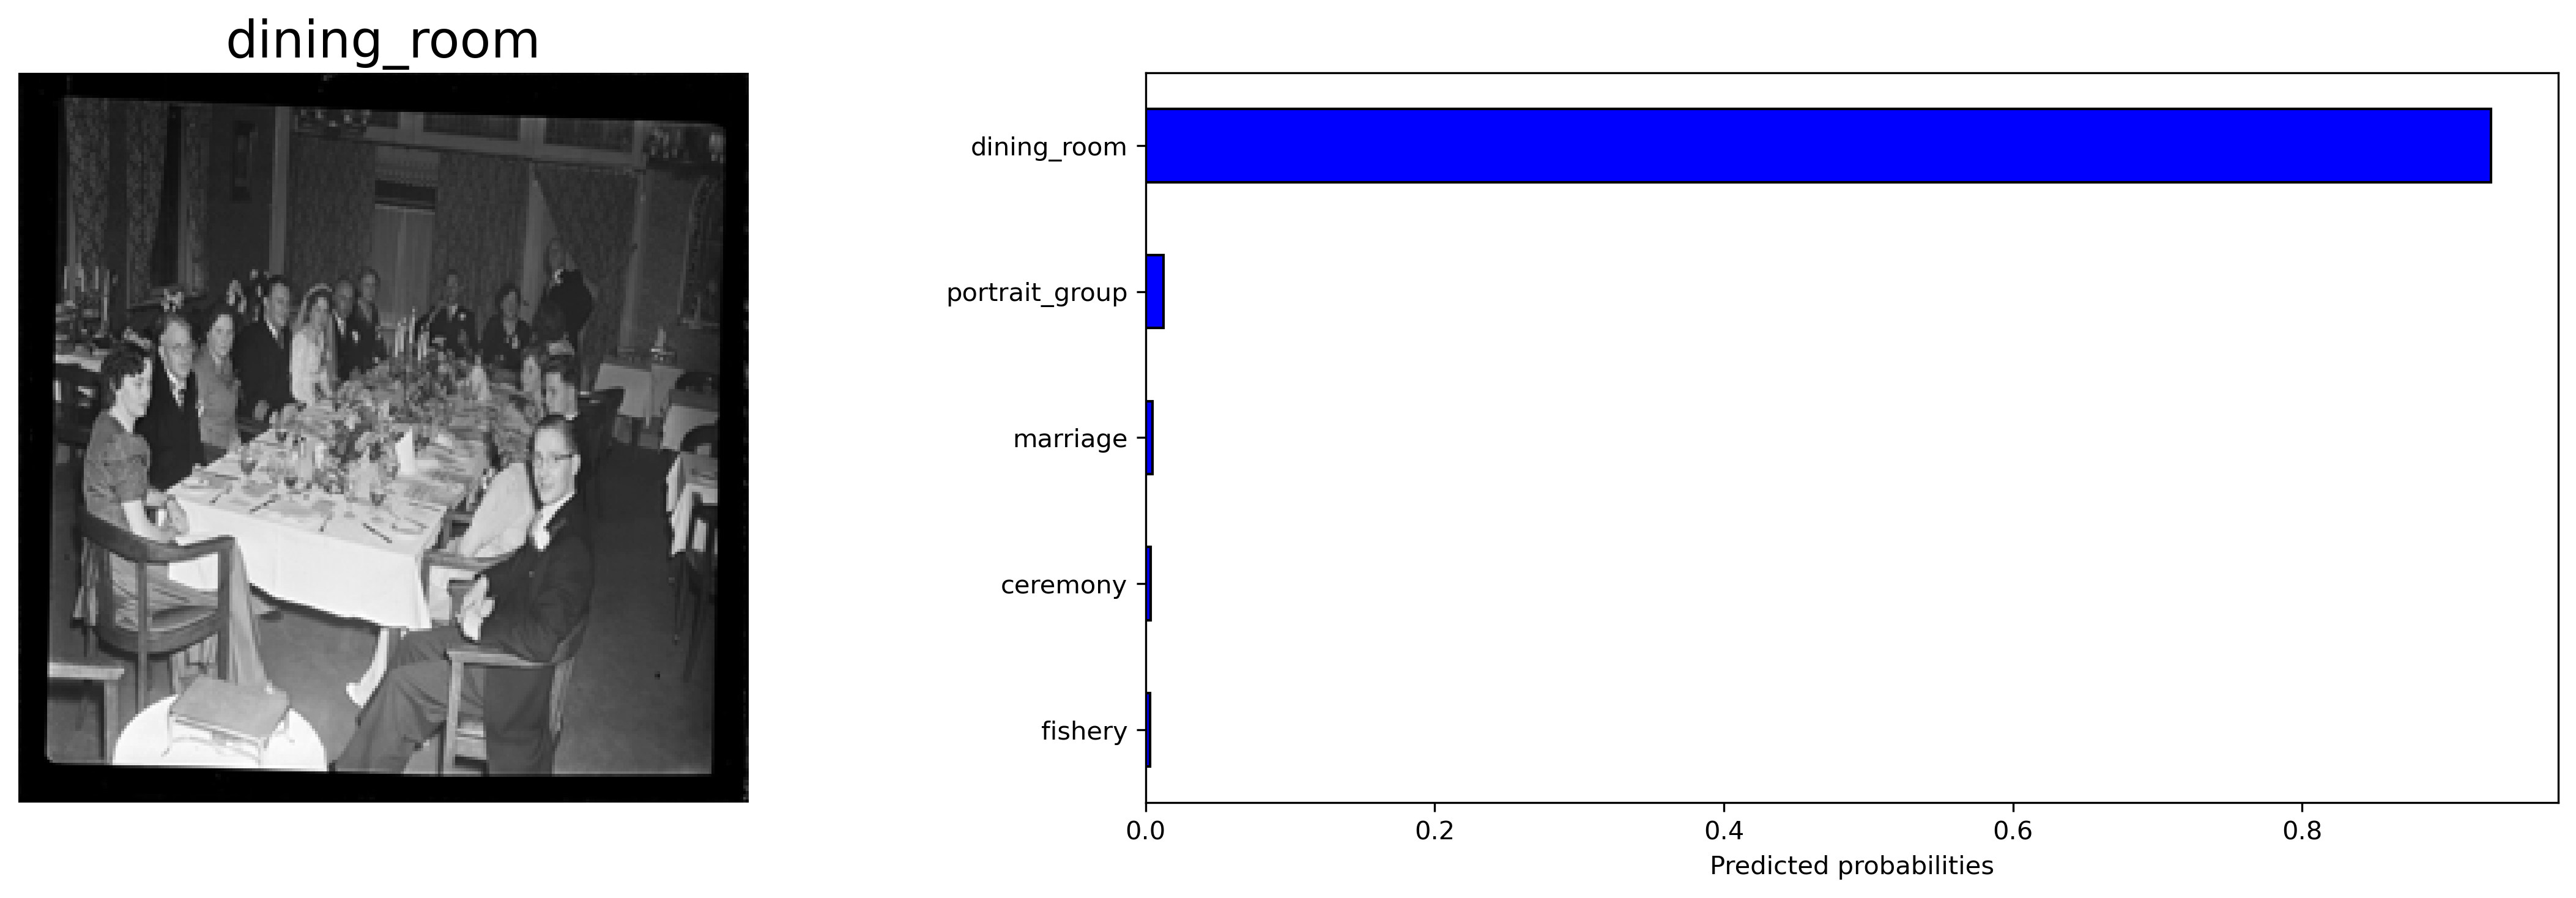
\includegraphics[width=\linewidth]{figures/dining_room.png}
 	\caption{Top-5 predictions for a picture with the label `Dining Room'.}
 	\label{fig:dining_room_example}
\end{figure}

\begin{figure}
	\centering
 	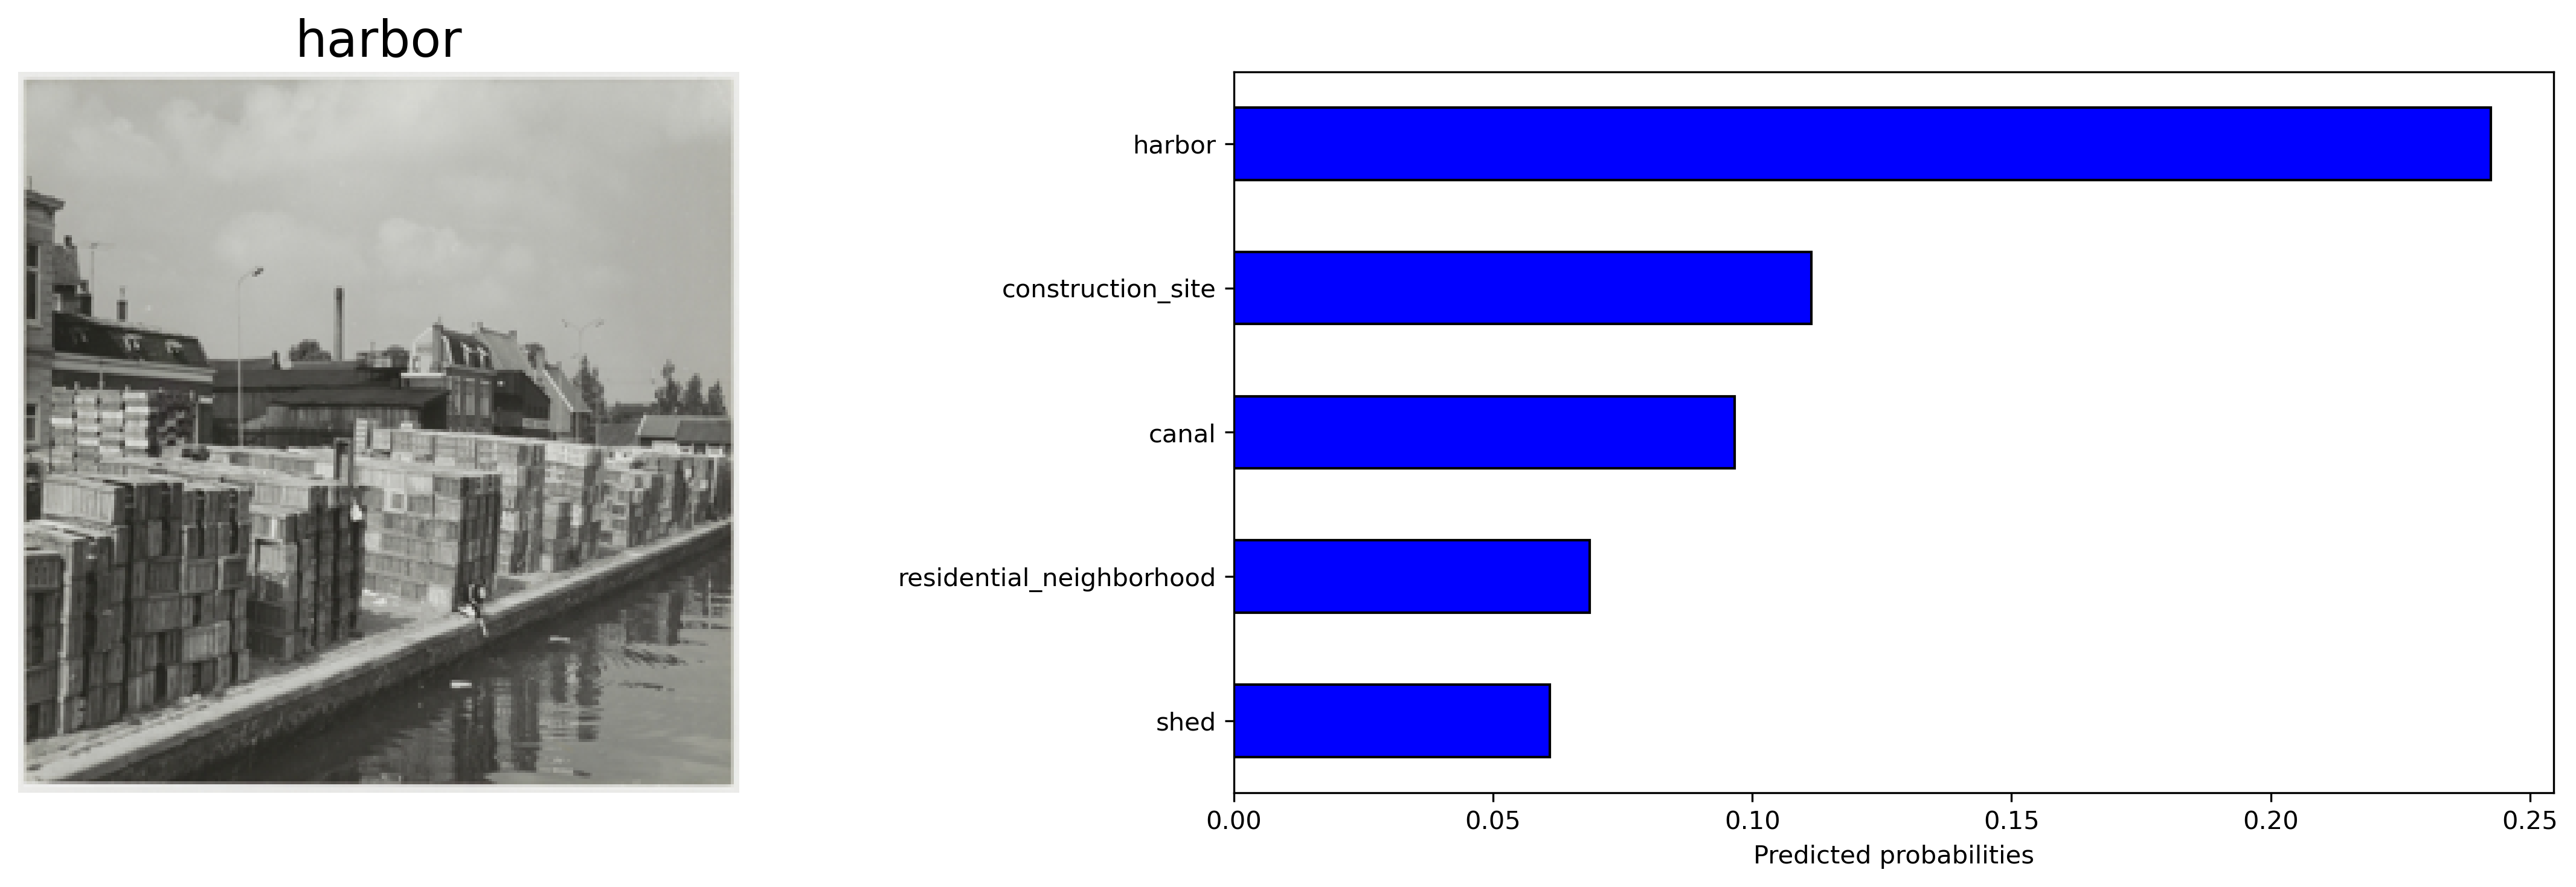
\includegraphics[width=\linewidth]{figures/harbor_example.png}
 	\caption{Top-5 predictions for a picture with the label `Harbor'.}
 	\label{fig:harbor_example}
\end{figure}


\begin{figure}
	\centering
 	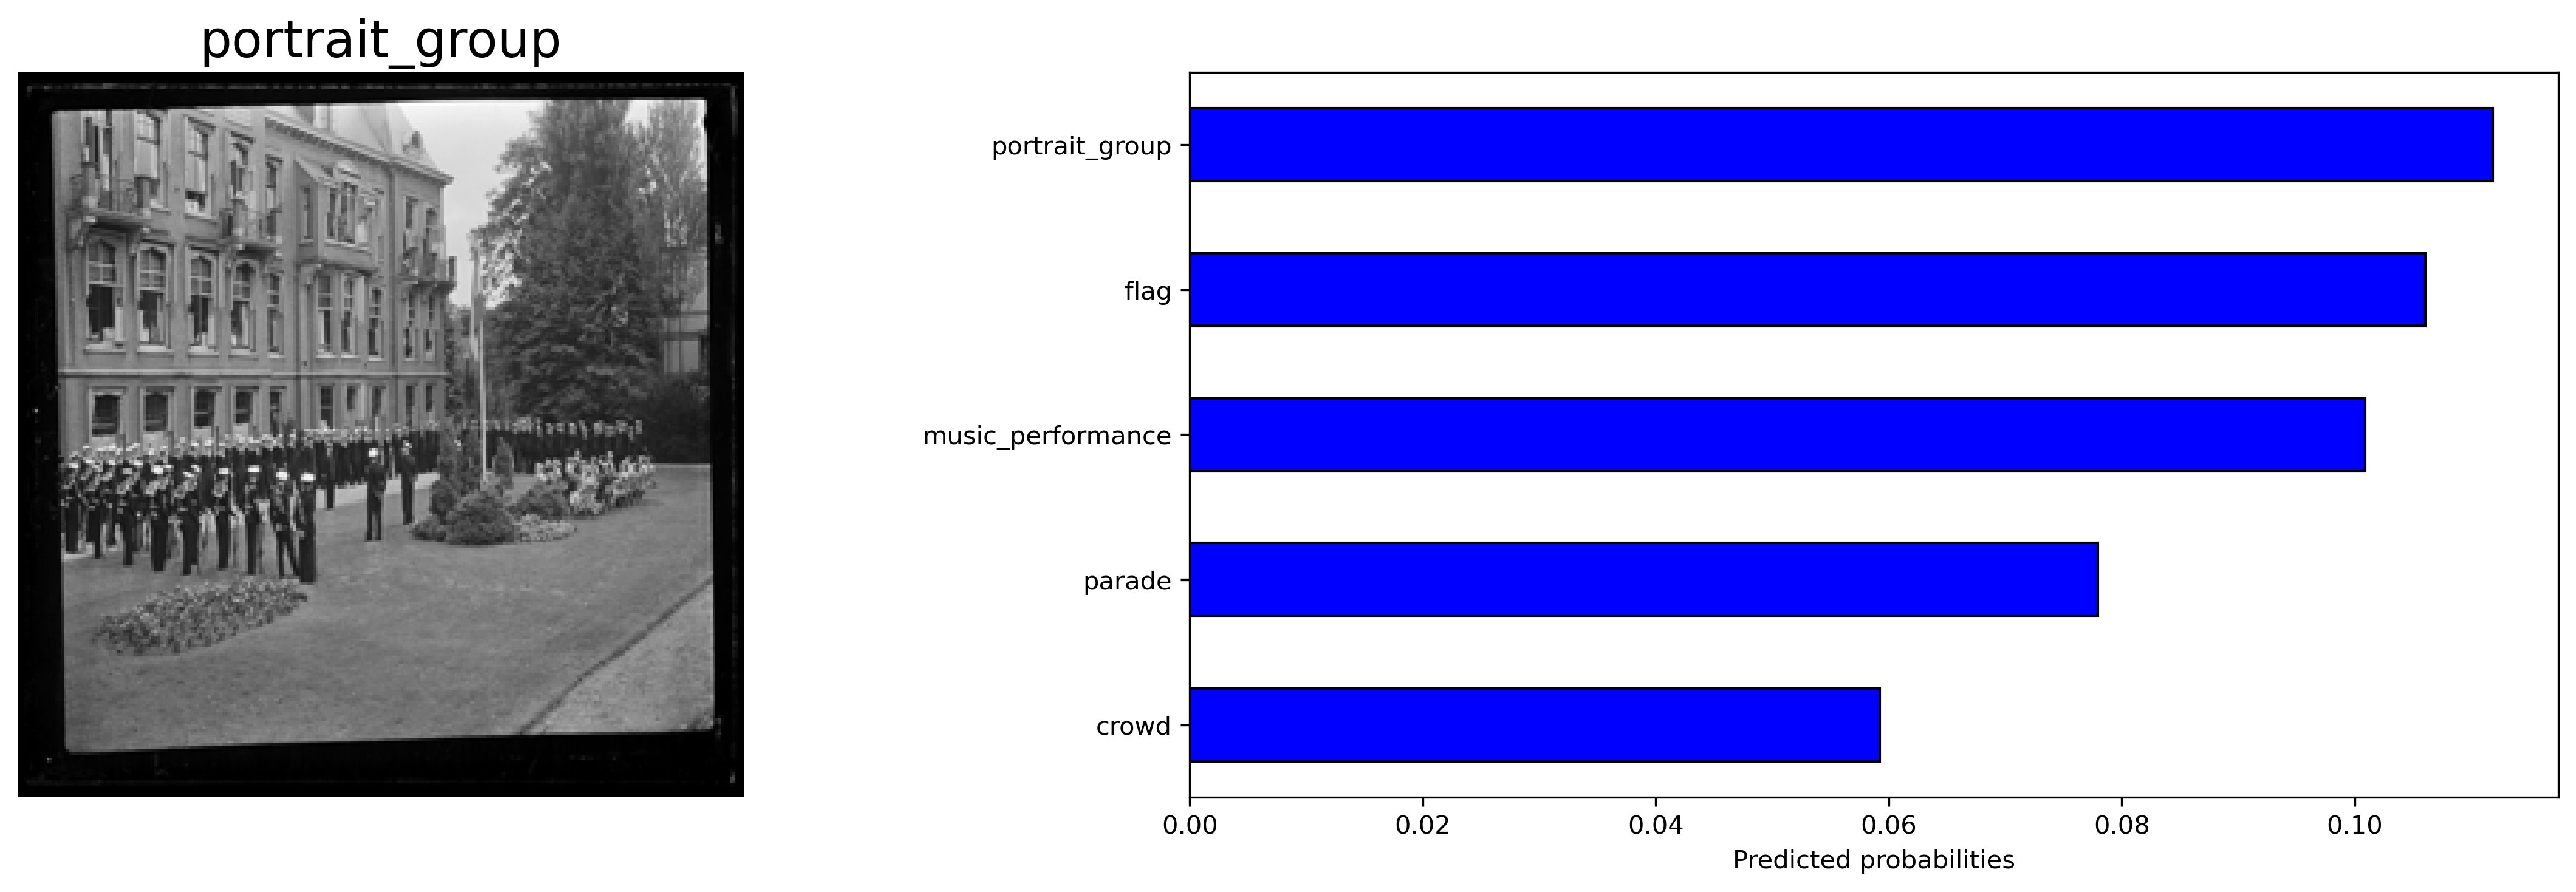
\includegraphics[width=\linewidth]{figures/portrait_group.png}
 	\caption{Top-5 predictions for a picture with the label `Portrait Group'.}
 	\label{fig:portrait_group_example}
\end{figure}


\begin{figure}
	\centering
 	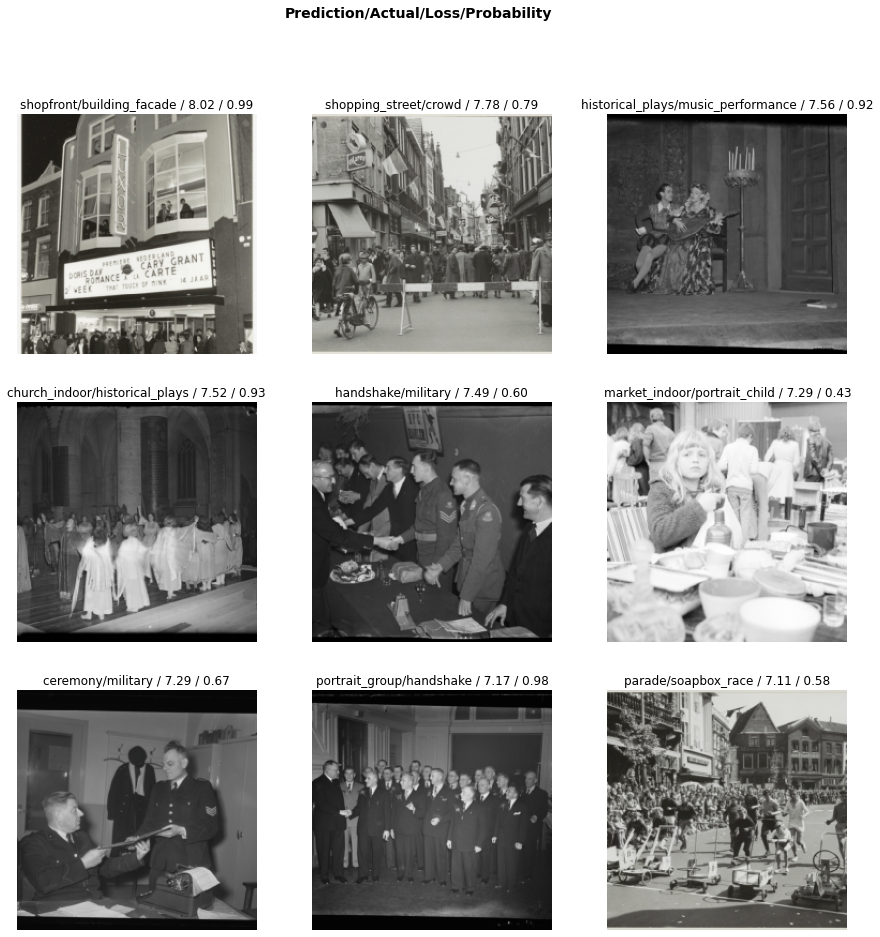
\includegraphics[width=\linewidth]{figures/top_losses.png}
 	\caption{Top Losses}
 	\label{fig:top_losses}
\end{figure}


\section{DISCUSSION}
\noindent This paper demonstrated how we annotated a data set of historical press photographs and applied transfer learning to leverage existing scene detection models to a new domain.
We highlighted the difficulties of categorization and possible solutions for working with skewed data sets. 
While our baseline model with basic image transformation already reached good accuracy scores, further augmentations including MixUp and Label Smoothing improved our top-1 accuracy (from 0.62 to 0.68). 
Our top-5 accuracy was only very slightly improved by these additional augmentations (0.88 to 0.89). 
The latter indicates that the correct answer was often among the top 5 answers given. While there still exists some ambiguity about labels, in some instances one of these five labels was understandable from a visual perspective, but it might cause some ethical concerns. 
For example, images of a funeral with lots of flowers were occasionally labelled as `parade'. 
Such mistakes are more impactful than mistaking, for instance, an automobile for a truck. In future work, we want to explore how we can penalize such mistakes; hence, improving the learning process. 
Furthermore, once more images of the collection have been digitized, we can further refine the presented model and improve and expand our presented categorization scheme.


\bibliographystyle{apalike}
{\small
\bibliography{bibliography.bib}


\section*{APPENDIX}
\label{sec:appendix}
\noindent Here we list our annotation guides lines per categories. Some of these categories have been not been included in the training, because they included fewer than twenty images. \\


\noindent\textbf{Accident Car} Traffic accident involving an automobile

\noindent\textbf{Accident Stretcher}
Accident involving an person on a stretcher

\noindent\textbf{Accident Train}
Traffic accident involving an train

\noindent\textbf{Aerial}
Picture with an aerial perspective

%\noindent\textbf{Airplane welcome}
%Pictures of people exiting a plane. These often included celebrities. 

\noindent\textbf{Amphitheater}
The collection contains many pictures taken at an outside amphitheater in Bloemendaal. 

\noindent\textbf{Animals cow}
Pictures of live and dead cows.

\noindent\textbf{Animals dog}
Pictures of dogs

\noindent\textbf{Animals horse}
Pictures of horses

\noindent\textbf{Animals misc}
Animals that do not fit in the previous categories. For final dataset, this might be subdivided in more categories.

\noindent\textbf{Artwork}
Artwork without people, the focus is on the art work.
There is also a separate category for statues. 

\noindent\textbf{Auditorium}
Public building (used for speeches, performances) where audience sits. Pictures with and without audiences. Overlap with categories `conference room` and `speech'

%\noindent\textbf{Badminton}
%People playing badminton

\noindent\textbf{Bakery}
Photos inside bakery, baking bread, presenting bread indoor/outdoors
Overlap with Kitchen

\noindent\textbf{Bar}
Area where drinks are served/consumed. Overlap with Dining Room/Game Room

\noindent\textbf{Baseball}
People playing baseball

%\noindent\textbf{Baseball team}
%Pictures of the baseball team, posing for a portrait.

\noindent\textbf{Basketball}
People playing basketball. 

%\noindent\textbf{Basketball team}
%Pictures of the basketball team, posing for a portrait.

\noindent\textbf{Beach}
If the beach is the picture's main focus, we select beach. Dunes is a separate category. Overlap with crowd/horse/running. When there is only water visible, we still select Beach. Possibly `sea' or `ocean' as a category.

%\noindent\textbf{Bedroom}
%Images taken within bedrooms, i.e. must feature a bed

\noindent\textbf{Beauty Salon}
Images that feature hairdressers or beauty salons

\noindent\textbf{Bicycles}
Features bicycles or people riding bicycles. Overlap with cycling, category for professional cycling and street/

\noindent\textbf{Boat Deck}
Picture that focus on the deck of a boat, either with or without people. Not showing entire ship/boat from a distance. Overlap with boats category.

\noindent\textbf{Boats}
Category focusing on a boat or multiple boats.
Overlap with harbor/shipyard. If boat is harboured and harbor is taking up large area of picture. Shipyard depicts construction area for boats, boats under construction
Overlap with beach, canal, river, waterfront. Difference is focus on boat

\noindent\textbf{Bookstore library}
Bookstore or library as a combined category, as they are often difficult to separate. The pictures feature rows of books and/or people reading.
Overlap with office, room which also often features books.

%\noindent\textbf{Bowling}
%People bowling
%
%\noindent\textbf{Boxing ring}
%Area for boxing matches.

\noindent\textbf{Bridge}
Picture should feature a bridge as a central element. Overlap with street/canal/river/boat

\noindent\textbf{Building Facade}
Depicting the facade of a building/rows of buildings. Not showing the full building from a distance. Overlap with residential area/mansion. Latter are single large house, former pictures of areas without a clear focus on the facade. Overlap shopping area/residential area/mansion

%\noindent\textbf{Bus Station}
%Area where busses depart. 
%
%\noindent\textbf{Bus Stop}
%Area where busses stop. 

\noindent\textbf{Bus/truck}
Focus on large busses and trucks. Overlap with street

\noindent\textbf{Butchers shop}
Butcher shop from inside, or people preparing meat. Overlap with animals/shopfront/shop/kitchen

%\noindent\textbf{Campsite}
%People camping using tents/caravans etc.

\noindent\textbf{Canal}
Flow of water, also includes natural flow of water rivers. Overlap with bridge/river/boat/fishing/waterfront

\noindent\textbf{Car}
Pictures that focus on a car

\noindent\textbf{Car shop}
Showroom in which cars are sold 

%\noindent\textbf{Casino}
%People gambling in a casino, playing black jack, slots, or roulette.
%
%\noindent\textbf{Castle}
%Pictures of a castle, or ruins of a castle.

\noindent\textbf{Catwalk}
Models on a catwalk

\noindent\textbf{Cemetery}
Pictures taken of a cemetery. Important element includes tombs, or tomb stones. 

\noindent\textbf{Ceremony}
A group of people bundled together for a ceremony. This could be awards, flowers, or a medal. Note that there is also a specific category for hand shakes. 

\noindent\textbf{Chess checkers}
People playing either chess or checkers. These are visually quite similar, for larger dataset, this category might be divided into two, if there are enough images.

\noindent\textbf{Church Indoor}
Pictures taken inside a church. This could include masses, but also view of the church without people. 

\noindent\textbf{Church Outdoor}
Pictures of the church/cathedral building.

\noindent\textbf{Circus}
Pictures taken of a circus, inside of a circus tent. The outside of the circus tent is categorized as tent. 

\noindent\textbf{City Hall Stairs}
Pictures taken of a group of people on the stairs outside of the city hall of Haarlem. This is quite a specific categories, but there are quite a few pictures that fit this category. 

\noindent\textbf{Classroom}
Students inside a classroom

\noindent\textbf{Clergy}
Pictures of clergy indoors or outdoors.

%\noindent\textbf{Coffin}
%Pictures of deceased people in a coffin. 

\noindent\textbf{Construction site}
Construction site, this also includes pictures of demolitions. It is quite difficult to separate the two visually. If enough images of both, we could separate the two. 

\noindent\textbf{Courtyard}
Area between buildings, or outside yard in a group of buildings. 

\noindent\textbf{Circus}
Pictures taken of a circus, inside of a circus tent. The outside of the circus tent is categorized as tent.  

\noindent\textbf{Cricket}
People playing cricket

%\noindent\textbf{Crosswalk}
%People crossing street, ‘zebra’ must be visible, otherwise street might be better

\noindent\textbf{Crowd}
Gathering of people, where individuals are not clearly discernible. When posing for picture put in portrait category.

\noindent\textbf{Cycling}
Professional cyclists

\noindent\textbf{Dancing}
People dancing
Overlap with bar, music performance, plaza

\noindent\textbf{Dining Room}
Area where people eat, both in restaurants and houses

%\noindent\textbf{Dorm room}
%Area with multiple beds, often bunk beds. 

\noindent\textbf{Drive Way}
Drive way in front of buildings

\noindent\textbf{Dunes}
Photos of dunes.
Overlap with parade/memorial/crowd

\noindent\textbf{Excavation}
People digging up something, archeological finds
Overlap with construction site

\noindent\textbf{Exhibition}
Room with artwork(s) and people. The focus is more clearly on the setting

\noindent\textbf{Factory indoor}
Pictures taken with factories/assembly lines/production facilities

%\noindent\textbf{Fair}
%Fun fairs

%\noindent\textbf{Farm}
%Buildings surrounded by pasture/animals/crops

\noindent\textbf{Farm field}
People working in farm fields/pictures of crops/farm fields
Overlap with animals

\noindent\textbf{Field Hockey}
People playing field hockey

%\noindent\textbf{Field hockey team}
%Pictures of field hockey teams

\noindent\textbf{Fire}
Pictures of fires, or building destroyed by fires. 

\noindent\textbf{Fishery}
Pictures of fishing industry

%\noindent\textbf{Fishing}
%People fishing

\noindent\textbf{Flag}
People holding or raising flags
Overlap with parade in which people hold flags

\noindent\textbf{Flowers}
Pictures that include flowers

\noindent\textbf{Forest/Park}
Picture taken in a forest or park

%\noindent\textbf{Fountain}
%Pictures of fountains

\noindent\textbf{Funeral}
Pictures of a funeral. Similar to memorial and cemetery. Here we only choose pictures that show a casket or burial itself.Overlap with memorial, parade, cemetery, flowers, church indoor

%\noindent\textbf{Garbage Dump}
%
%\noindent\textbf{Gas Station}

\noindent\textbf{Gymnastics}
People performing gymnastics indoor and outdoor
Overlap with circus/dancing

\noindent\textbf{Handshake}
People shaking hands, subcategory of ceremony. 

\noindent\textbf{Harbor}
Ships docked at a harbor, focus is not ships, but context of the harbor. 
Overlap with boats and waterfront > waterfront is focus is on waterfront/kade

\noindent\textbf{Historical plays}
People dressed up in historical garment enacting historical plays


\noindent\textbf{Hospital}
Pictures taken in a hospital/dentist/medical lab setting

%\noindent\textbf{House Boat}
%Pictures of the outside of house boats.

\noindent\textbf{Ice Skating}
People skating on ice

\noindent\textbf{Kitchen}
People in kitchen, preparing food
Overlap with butcher\_store

%\noindent\textbf{Korfbal}
%People playing korfbal, a dutch variant of basketball.
%
%\noindent\textbf{Laboratory}
%
%\noindent\textbf{Lighthouse}

\noindent\textbf{Living room}
People situated in a living room space.
Overlap with portraits, which are often taken in a living room. To learn the living room category, I placed pictures in here taken in living rooms, with enough information on the living room. Overlap with portrait

\noindent\textbf{Mansion}
Large houses, separated from housing blocks

\noindent\textbf{Market indoor}
Indoor market/shopping fair

\noindent\textbf{Market outdoor}
Outdoor market
Overlap with crowd

\noindent\textbf{Marriage}
Depicting a marriage couple, marriage ceremony
Overlap with portrait group

%\noindent\textbf{Martial Arts Gym}
%Space where people fight, judo/karate

\noindent\textbf{Meeting Room}
Setting features meeting table with people sitting around it

\noindent\textbf{Memorial}
Depicting a memorial site. Overlap with funeral/flowers/flag

\noindent\textbf{Military}
Pictures depicting military personnel or military equipment. Overlap with parade and bus/trucks

\noindent\textbf{Motorcycle}
Depicting motorcycle(s)

%\noindent\textbf{Movie set}
%Depicting movie sets

\noindent\textbf{Musical Performance}
People performing music
Overlap with dance

\noindent\textbf{Office}
Pictures set in an office environment

\noindent\textbf{Parade}
People parading, marching bands

\noindent\textbf{Parade floats}
Pictures with flower trucks/floats

\noindent\textbf{Patio}
People on patio’s sitting

\noindent\textbf{Playground}
People/Children playing in a playground. Overlap with funfair and portrait children

%\noindent\textbf{Playing Cards}
%People playing cards

\noindent\textbf{Pond}
Scenery of a pond. Overlap with canal/river/park

\noindent\textbf{Portrait Child}
One child

\noindent\textbf{Portrait Children}
More children

\noindent\textbf{Portrait Individual}

\noindent\textbf{Portrait Group}

\noindent\textbf{Protest}
People protesting, banners clear signal

\noindent\textbf{Racecourse}
Pictures taken on racecourse. Also category soapbox race
Overlap with car, accident. 

%\noindent\textbf{Railroad track}
%Pictures of the railroad track. There’s is also a category for trains.
%
%\noindent\textbf{Repair Shop}
%Indoor pictures of repair shop, showing person repairing objects

\noindent\textbf{Residential neighborhood}
Living area. Overlap with street/building facade

\noindent\textbf{Rowing}
People rowing

\noindent\textbf{Running}
People running in a sports event

\noindent\textbf{Saint Niclaus}
Pictures of the Saint Niclaus festivities

\noindent\textbf{Shed}
Wooden buildings, beach houses, living trailers

\noindent\textbf{Shipyard}
Construction area for ships. Overlap with boats and harbor. 

\noindent\textbf{Shop interior}
Photos of different kinds of shop interiors. 

\noindent\textbf{Shop front}
Picture of a shop front, ‘etalage’

\noindent\textbf{Shopping street}
Depicting street of shops/shoppers

\noindent\textbf{Sign}
Signs, plaques, maps

%\noindent\textbf{Snooker}
%People playing snooker, or billiards.

\noindent\textbf{Snowfield}
Scenes set in snow, people skiing, sledding

\noindent\textbf{Soapbox Race}

\noindent\textbf{Soccer}
people playing soccer

\noindent\textbf{Soccer Indoor}
People playing indoor soccer

\noindent\textbf{Soccer Team}
Portrait of soccer team

\noindent\textbf{Speech}
Focus on person specking

\noindent\textbf{Statue}
Pictures of sculptures/statues

\noindent\textbf{Street}
Depicting street sceneries. Overlap with car, residential neighbourhood 

%\noindent\textbf{Surfing}
%Depicting street sceneries. Overlap with car, residential neighbourhood 

\noindent\textbf{Swimming Pool Indoor}

\noindent\textbf{Swimming Pool Outdoor}

%\noindent\textbf{Swimming Team}
%Portrait of a swimming team
%
%\noindent\textbf{Table Tennis}
%
%\noindent\textbf{Telecom}
%Pictures taken in radio studios, switchboards etc.
%
%\noindent\textbf{Tent}
%Large tents, small tents should be placed in category campsite.

\noindent\textbf{Theatre}
Plays performed in a theatre setting

\noindent\textbf{Tower}
Pictures of towers, not church towers. 

\noindent\textbf{Train}
Pictures of trains. Overlap with train station

%\noindent\textbf{Train interior}
%Pictures of interiors of trains.

\noindent\textbf{Train station}
Pictures of train stations, trains at stations etc..

\noindent\textbf{Tram}
Pictures of trams

\noindent\textbf{Volley ball}
Pictures of people playing volley ball

%\noindent\textbf{Water Polo}
%People playing water polo

\noindent\textbf{Water ski}
People on water skis

\noindent\textbf{Water Front}
Scenes that focus on the water front

\noindent\textbf{Windmill}
Pictures that contain a windmill


\noindent If any, the appendix should appear directly after the
references without numbering, and not on a new page. To do so please use the following command:


\end{document}

